\documentclass[]{book}
\usepackage{lmodern}
\usepackage{amssymb,amsmath}
\usepackage{ifxetex,ifluatex}
\usepackage{fixltx2e} % provides \textsubscript
\ifnum 0\ifxetex 1\fi\ifluatex 1\fi=0 % if pdftex
  \usepackage[T1]{fontenc}
  \usepackage[utf8]{inputenc}
\else % if luatex or xelatex
  \ifxetex
    \usepackage{mathspec}
  \else
    \usepackage{fontspec}
  \fi
  \defaultfontfeatures{Ligatures=TeX,Scale=MatchLowercase}
\fi
% use upquote if available, for straight quotes in verbatim environments
\IfFileExists{upquote.sty}{\usepackage{upquote}}{}
% use microtype if available
\IfFileExists{microtype.sty}{%
\usepackage{microtype}
\UseMicrotypeSet[protrusion]{basicmath} % disable protrusion for tt fonts
}{}
\usepackage[margin=1in]{geometry}
\usepackage{hyperref}
\hypersetup{unicode=true,
            pdftitle={Data Science Course in a Box},
            pdfauthor={Mine Çetinkaya-Rundel},
            pdfborder={0 0 0},
            breaklinks=true}
\urlstyle{same}  % don't use monospace font for urls
\usepackage{natbib}
\bibliographystyle{apalike}
\usepackage{color}
\usepackage{fancyvrb}
\newcommand{\VerbBar}{|}
\newcommand{\VERB}{\Verb[commandchars=\\\{\}]}
\DefineVerbatimEnvironment{Highlighting}{Verbatim}{commandchars=\\\{\}}
% Add ',fontsize=\small' for more characters per line
\usepackage{framed}
\definecolor{shadecolor}{RGB}{248,248,248}
\newenvironment{Shaded}{\begin{snugshade}}{\end{snugshade}}
\newcommand{\KeywordTok}[1]{\textcolor[rgb]{0.13,0.29,0.53}{\textbf{#1}}}
\newcommand{\DataTypeTok}[1]{\textcolor[rgb]{0.13,0.29,0.53}{#1}}
\newcommand{\DecValTok}[1]{\textcolor[rgb]{0.00,0.00,0.81}{#1}}
\newcommand{\BaseNTok}[1]{\textcolor[rgb]{0.00,0.00,0.81}{#1}}
\newcommand{\FloatTok}[1]{\textcolor[rgb]{0.00,0.00,0.81}{#1}}
\newcommand{\ConstantTok}[1]{\textcolor[rgb]{0.00,0.00,0.00}{#1}}
\newcommand{\CharTok}[1]{\textcolor[rgb]{0.31,0.60,0.02}{#1}}
\newcommand{\SpecialCharTok}[1]{\textcolor[rgb]{0.00,0.00,0.00}{#1}}
\newcommand{\StringTok}[1]{\textcolor[rgb]{0.31,0.60,0.02}{#1}}
\newcommand{\VerbatimStringTok}[1]{\textcolor[rgb]{0.31,0.60,0.02}{#1}}
\newcommand{\SpecialStringTok}[1]{\textcolor[rgb]{0.31,0.60,0.02}{#1}}
\newcommand{\ImportTok}[1]{#1}
\newcommand{\CommentTok}[1]{\textcolor[rgb]{0.56,0.35,0.01}{\textit{#1}}}
\newcommand{\DocumentationTok}[1]{\textcolor[rgb]{0.56,0.35,0.01}{\textbf{\textit{#1}}}}
\newcommand{\AnnotationTok}[1]{\textcolor[rgb]{0.56,0.35,0.01}{\textbf{\textit{#1}}}}
\newcommand{\CommentVarTok}[1]{\textcolor[rgb]{0.56,0.35,0.01}{\textbf{\textit{#1}}}}
\newcommand{\OtherTok}[1]{\textcolor[rgb]{0.56,0.35,0.01}{#1}}
\newcommand{\FunctionTok}[1]{\textcolor[rgb]{0.00,0.00,0.00}{#1}}
\newcommand{\VariableTok}[1]{\textcolor[rgb]{0.00,0.00,0.00}{#1}}
\newcommand{\ControlFlowTok}[1]{\textcolor[rgb]{0.13,0.29,0.53}{\textbf{#1}}}
\newcommand{\OperatorTok}[1]{\textcolor[rgb]{0.81,0.36,0.00}{\textbf{#1}}}
\newcommand{\BuiltInTok}[1]{#1}
\newcommand{\ExtensionTok}[1]{#1}
\newcommand{\PreprocessorTok}[1]{\textcolor[rgb]{0.56,0.35,0.01}{\textit{#1}}}
\newcommand{\AttributeTok}[1]{\textcolor[rgb]{0.77,0.63,0.00}{#1}}
\newcommand{\RegionMarkerTok}[1]{#1}
\newcommand{\InformationTok}[1]{\textcolor[rgb]{0.56,0.35,0.01}{\textbf{\textit{#1}}}}
\newcommand{\WarningTok}[1]{\textcolor[rgb]{0.56,0.35,0.01}{\textbf{\textit{#1}}}}
\newcommand{\AlertTok}[1]{\textcolor[rgb]{0.94,0.16,0.16}{#1}}
\newcommand{\ErrorTok}[1]{\textcolor[rgb]{0.64,0.00,0.00}{\textbf{#1}}}
\newcommand{\NormalTok}[1]{#1}
\usepackage{longtable,booktabs}
\usepackage{graphicx,grffile}
\makeatletter
\def\maxwidth{\ifdim\Gin@nat@width>\linewidth\linewidth\else\Gin@nat@width\fi}
\def\maxheight{\ifdim\Gin@nat@height>\textheight\textheight\else\Gin@nat@height\fi}
\makeatother
% Scale images if necessary, so that they will not overflow the page
% margins by default, and it is still possible to overwrite the defaults
% using explicit options in \includegraphics[width, height, ...]{}
\setkeys{Gin}{width=\maxwidth,height=\maxheight,keepaspectratio}
\IfFileExists{parskip.sty}{%
\usepackage{parskip}
}{% else
\setlength{\parindent}{0pt}
\setlength{\parskip}{6pt plus 2pt minus 1pt}
}
\setlength{\emergencystretch}{3em}  % prevent overfull lines
\providecommand{\tightlist}{%
  \setlength{\itemsep}{0pt}\setlength{\parskip}{0pt}}
\setcounter{secnumdepth}{5}
% Redefines (sub)paragraphs to behave more like sections
\ifx\paragraph\undefined\else
\let\oldparagraph\paragraph
\renewcommand{\paragraph}[1]{\oldparagraph{#1}\mbox{}}
\fi
\ifx\subparagraph\undefined\else
\let\oldsubparagraph\subparagraph
\renewcommand{\subparagraph}[1]{\oldsubparagraph{#1}\mbox{}}
\fi

%%% Use protect on footnotes to avoid problems with footnotes in titles
\let\rmarkdownfootnote\footnote%
\def\footnote{\protect\rmarkdownfootnote}

%%% Change title format to be more compact
\usepackage{titling}

% Create subtitle command for use in maketitle
\newcommand{\subtitle}[1]{
  \posttitle{
    \begin{center}\large#1\end{center}
    }
}

\setlength{\droptitle}{-2em}
  \title{Data Science Course in a Box}
  \pretitle{\vspace{\droptitle}\centering\huge}
  \posttitle{\par}
  \author{Mine Çetinkaya-Rundel}
  \preauthor{\centering\large\emph}
  \postauthor{\par}
  \predate{\centering\large\emph}
  \postdate{\par}
  \date{2018-04-23}

\usepackage{booktabs}
\usepackage{amsthm}
\makeatletter
\def\thm@space@setup{%
  \thm@preskip=8pt plus 2pt minus 4pt
  \thm@postskip=\thm@preskip
}
\makeatother

\usepackage{amsthm}
\newtheorem{theorem}{Theorem}[chapter]
\newtheorem{lemma}{Lemma}[chapter]
\theoremstyle{definition}
\newtheorem{definition}{Definition}[chapter]
\newtheorem{corollary}{Corollary}[chapter]
\newtheorem{proposition}{Proposition}[chapter]
\theoremstyle{definition}
\newtheorem{example}{Example}[chapter]
\theoremstyle{definition}
\newtheorem{exercise}{Exercise}[chapter]
\theoremstyle{remark}
\newtheorem*{remark}{Remark}
\newtheorem*{solution}{Solution}
\begin{document}
\maketitle

{
\setcounter{tocdepth}{1}
\tableofcontents
}
\chapter*{Welcome}\label{welcome}
\addcontentsline{toc}{chapter}{Welcome}

Some welcome words\ldots{}

\chapter{Introduction}\label{intro}

This is not a book per se, at least not yet. It's a place for organizing
materials for teaching (and learning) data science with R, RStudio, the
tidyverse and tidyverse friendly packages. It's called \textbf{Data
Science Course in a Box}, as it contains all the materials you (an
educator) might need to teach data science or you (a learner) might find
useful to learn about them.

\section{Who is this course for?}\label{who-is-this-course-for}

The materials in this box are designed for learners who have no
background in data science, statistics, or programming. However, they
also assume that the learners are interested in making sense of
(sometimes messy) data and willing to dive into the documentation of the
packages we introduce.

\section{What is in the box?}\label{what-is-in-the-box}

\begin{itemize}
\tightlist
\item
  Slides
\item
  Labs
\item
  Assignments
\item
  Exams
\item
  Infrastructure guide
\end{itemize}

\section{How is the course content
organized?}\label{how-is-the-course-content-organized}

\begin{itemize}
\tightlist
\item
  Part 1: Exploring data - wrangle + visualize + collect
\item
  Part 2: Making rigorous conclusions - modeling + inference
\item
  Part 3: Looking forward - \ldots{}
\end{itemize}

\section{Why R?}\label{why-r}

Unlike most other software designed specifically for teaching
statistics, R is free and open source, powerful, flexible, and relevant
beyond the introductory statistics classroom. Arguments against using
and teaching R at especially the introductory statistics level generally
cluster around the following two points: teaching programming in
addition to statistical concepts is challenging and the command line is
more intimidating to beginners than the graphical user interface (GUI)
most point-and-click type software offer.

One solution for these concerns is to avoid hands-on data analysis
completely. If we do not ask our students to start with raw data and
instead always provide them with small, tidy rectangles of data then
there is never really a need for statistical software beyond spreadsheet
or graphing calculator. This is not what we want in a modern statistics
course and is a disservice to students.

Another solution is to use traditional point-and-click software for data
analysis. The typical argument is that the GUI is easier for students to
learn and so they can spend more time on statistical concepts. However,
this ignores the fact that these software tools also have nontrivial
learning curves. In fact, teaching specific data analysis tasks using
such software often requires lengthy step-by-step instructions, with
annotated screenshots, for navigating menus and other interface
elements. Also, it is not uncommon that instructions for one task do not
easily extend to another. Replacing such instructions with just a few
lines of R code actually makes the instructional materials more concise
and less intimidating.

Many in the statistics education community are in favor of teaching R
(or some other programming language, like Python) in upper level
statistics courses, however the value of using R in introductory
statistics courses is not as widely accepted. We acknowledge that this
addition can be burdensome, however we would argue that learning a tool
that is applicable beyond the introductory statistics course and that
enhances students' problem solving skills is a burden worth bearing.

\section{Why RStudio?}\label{why-rstudio}

The RStudio IDE includes a viewable environment, a file browser, data
viewer, and a plotting pane, which makes it less intimidating than the
bare R shell. Additionally, since it is a full fledged IDE, it also
features integrated help, syntax highlighting, and context-aware tab
completion, which are all powerful tools that help flatten the learning
curve.

Students access the RStudio IDE through a centralized RStudio server
instance, which allows us to provide students with uniform computing
environments. Additionally, RStudio's direct integration with other
critically important tools for teaching computing best practices and
reproducible research also influenced our decision for making it central
in our toolkit.

It should be noted that we do not want to completely dissuade students
from downloading and installing R and RStudio locally, we just do not
want it to be a prerequisite for getting started. We have found that
teaching personal setup is best done progressively throughout a
semester, usually via one-on-one interactions during office hours or
after class. Our goal is that all students will be able to continue
using R even if they no longer have access to departmental resources.

\chapter{Setup}\label{setup}

There are four things you need to run the code in this book: R, RStudio,
a collection of R packages called the \textbf{tidyverse}, and a handful
of other packages. Packages are the fundamental units of reproducible R
code. They include reusable functions, the documentation that describes
how to use them, and sample data.

\section{On the Cloud}\label{on-the-cloud}

You can access all on the cloud, via
\href{http://rstudio.cloud/}{RStudio Cloud}, and avoid local
installation.

See \href{https://rstudio.cloud/spaces/1655/projects}{RStudio Cloud
workspace} that you can copy (soon?) for your course.

\section{Locally}\label{locally}

{[}SOME OF WHAT'S BELOW IS BORROWED FROM R4DS AND HERE AS A PLACEHOLDER
AND WILL BE REVISED AND REMOVED.{]}

\subsection{R}\label{r}

To download R, go to CRAN, the \textbf{c}omprehensive \textbf{R}
\textbf{a}rchive \textbf{n}etwork. CRAN is composed of a set of mirror
servers distributed around the world and is used to distribute R and R
packages. Don't try and pick a mirror that's close to you: instead use
the cloud mirror, \url{https://cloud.r-project.org}, which automatically
figures it out for you.

A new major version of R comes out once a year, and there are 2-3 minor
releases each year. It's a good idea to update regularly. Upgrading can
be a bit of a hassle, especially for major versions, which require you
to reinstall all your packages, but putting it off only makes it worse.

\subsection{RStudio}\label{rstudio}

{[}TO DO: THERE ARE SOME WORDS BORROWED FROM R4DS BELOW, CLEAN THEM
UP.{]}

RStudio is an integrated development environment, or IDE, for R
programming. Download and install it from
\url{http://www.rstudio.com/download}. RStudio is updated a couple of
times a year. When a new version is available, RStudio will let you
know. It's a good idea to upgrade regularly so you can take advantage of
the latest and greatest features.

\subsection{The tidyverse}\label{the-tidyverse}

You'll also need to install some R packages. An R \textbf{package} is a
collection of functions, data, and documentation that extends the
capabilities of base R. Using packages is key to the successful use of
R. The majority of the packages that you will learn in this book are
part of the so-called tidyverse. The packages in the tidyverse share a
common philosophy of data and R programming, and are designed to work
together naturally.

You can install the complete tidyverse with a single line of code:

\begin{Shaded}
\begin{Highlighting}[]
\KeywordTok{install.packages}\NormalTok{(}\StringTok{"tidyverse"}\NormalTok{)}
\end{Highlighting}
\end{Shaded}

On your own computer, type that line of code in the console, and then
press enter to run it. R will download the packages from CRAN and
install them on to your computer. If you have problems installing, make
sure that you are connected to the internet, and that
\url{https://cloud.r-project.org/} isn't blocked by your firewall or
proxy.

You will not be able to use the functions, objects, and help files in a
package until you load it with \texttt{library()}. Once you have
installed a package, you can load it with the \texttt{library()}
function:

\begin{Shaded}
\begin{Highlighting}[]
\KeywordTok{library}\NormalTok{(tidyverse)}
\CommentTok{#> -- Attaching packages ------------------- tidyverse 1.2.1 --}
\CommentTok{#> √ ggplot2 2.2.1          √ purrr   0.2.4     }
\CommentTok{#> √ tibble  1.4.2          √ dplyr   0.7.4.9002}
\CommentTok{#> √ tidyr   0.8.0          √ stringr 1.3.0     }
\CommentTok{#> √ readr   1.1.1          √ forcats 0.3.0}
\CommentTok{#> -- Conflicts ---------------------- tidyverse_conflicts() --}
\CommentTok{#> x dplyr::filter() masks stats::filter()}
\CommentTok{#> x dplyr::lag()    masks stats::lag()}
\end{Highlighting}
\end{Shaded}

This tells you that tidyverse is loading the ggplot2, tibble, tidyr,
readr, purrr, and dplyr packages. These are considered to be the
\textbf{core} of the tidyverse because you'll use them in almost every
analysis.

Packages in the tidyverse change fairly frequently. You can see if
updates are available, and optionally install them, by running
\texttt{tidyverse\_update()}.

\subsection{Other packages}\label{other-packages}

There are many other excellent packages that are not part of the
tidyverse, because they solve problems in a different domain, or are
designed with a different set of underlying principles. This doesn't
make them better or worse, just different. In other words, the
complement to the tidyverse is not the messyverse, but many other
universes of interrelated packages. As you tackle more data science
projects with R, you'll learn new packages and new ways of thinking
about data.

In this book we'll use three data packages from outside the tidyverse:

\begin{Shaded}
\begin{Highlighting}[]
\KeywordTok{install.packages}\NormalTok{(}\KeywordTok{c}\NormalTok{(}\StringTok{"nycflights13"}\NormalTok{, }\StringTok{"fivethirtyeight"}\NormalTok{))}
\end{Highlighting}
\end{Shaded}

{[}TO DO: ADD OTHERS{]}

These packages provide data on airline flights, world development, and
baseball that we'll use to illustrate key data science ideas.

\chapter{Day one}\label{dayone}

You only get one first day of class, so start with something that
excites students, teach the necessary evils later. This means getting to
a meaningful, and hopefully interesting (for the students) data
visualization as quickly as possible.

\section{What is data science?}\label{what-is-data-science}

Data science is an exciting discipline that allows you to turn raw data
into understanding, insight, and knowledge. We're going to learn to do
this in a \texttt{tidy} way -- more on that later!

\section{What is this course?}\label{what-is-this-course}

This is an introductory data science course designed for learners with
no background in data science, programming, or statistics, but a
willingness to learn in class and explore independently.

\begin{itemize}
\tightlist
\item
  Will we be doing computing? Yes.
\item
  Is this an intro CS course? Not really, but many themes are shared.
\item
  Is this an intro stat course? In a way, but it's not your high school
  statistics course.
\item
  What computing language will we learn? R.
\item
  Why not language X? We can discuss that over :coffee:.
\end{itemize}

\section{Data in the wild}\label{data-in-the-wild}

I like starting off by showing a few examples of easy to follow but not
so simple data analyses done in R, preferably presented along with the R
code. This should be the type of analysis they could do for their final
project. Blog posts are often good examples for these. In Spring 2018 I
used the following as examples:

\begin{itemize}
\tightlist
\item
  \href{http://livefreeordichotomize.com/2017/12/27/a-year-as-told-by-fitbit/}{A
  year as told by fitbit} by Nick Strayer
\item
  \href{http://www.masalmon.eu/2017/10/06/globalrladiestour/}{R-Ladies
  global tour} by Maelle Salmon
\item
  \href{http://varianceexplained.org/r/trump-tweets/}{Text analysis of
  Trump's tweets confirms he writes only the (angrier) Android half} by
  David Robinson
\end{itemize}

\section{Your turn: UN Votes}\label{your-turn-un-votes}

It's now time to let the students work on their first data visualization
in R.

Using the \texttt{unvotes} package, and a pre-populated R Markdown
document on RStudio Cloud, they can create and modify the two
multi-variate plots, visualizing the voting history of countries in the
United Nations General Assembly.

\begin{Shaded}
\begin{Highlighting}[]
\KeywordTok{library}\NormalTok{(unvotes)}
\CommentTok{#> If you use data from the unvotes package, please cite the following:}
\CommentTok{#> }
\CommentTok{#> Erik Voeten "Data and Analyses of Voting in the UN General Assembly" Routledge Handbook of International Organization, edited by Bob Reinalda (published May 27, 2013)}
\KeywordTok{library}\NormalTok{(tidyverse)}
\CommentTok{#> -- Attaching packages ------------------- tidyverse 1.2.1 --}
\CommentTok{#> √ ggplot2 2.2.1          √ purrr   0.2.4     }
\CommentTok{#> √ tibble  1.4.2          √ dplyr   0.7.4.9002}
\CommentTok{#> √ tidyr   0.8.0          √ stringr 1.3.0     }
\CommentTok{#> √ readr   1.1.1          √ forcats 0.3.0}
\CommentTok{#> -- Conflicts ---------------------- tidyverse_conflicts() --}
\CommentTok{#> x dplyr::filter() masks stats::filter()}
\CommentTok{#> x dplyr::lag()    masks stats::lag()}
\KeywordTok{library}\NormalTok{(lubridate)}
\CommentTok{#> Loading required package: methods}
\CommentTok{#> }
\CommentTok{#> Attaching package: 'lubridate'}
\CommentTok{#> The following object is masked from 'package:base':}
\CommentTok{#> }
\CommentTok{#>     date}
\end{Highlighting}
\end{Shaded}

We will narrow down the analysis to four countries: United States,
Russian Federation, Mexico, and Turkey.

\begin{Shaded}
\begin{Highlighting}[]
\NormalTok{country_list <-}\StringTok{ }\KeywordTok{c}\NormalTok{(}\StringTok{"United States of America"}\NormalTok{, }\StringTok{"Russian Federation"}\NormalTok{, }
                  \StringTok{"Mexico"}\NormalTok{, }\StringTok{"Turkey"}\NormalTok{)}
\end{Highlighting}
\end{Shaded}

First we take a look at how often each country voted ``yes'' on a
resolution in each year.

\begin{Shaded}
\begin{Highlighting}[]
\NormalTok{un_votes }\OperatorTok
\StringTok{  }\KeywordTok{filter}\NormalTok{(country }\OperatorTok\StringTok{ }\NormalTok{country_list) }\OperatorTok
\StringTok{  }\KeywordTok{inner_join}\NormalTok{(un_roll_calls, }\DataTypeTok{by =} \StringTok{"rcid"}\NormalTok{) }\OperatorTok
\StringTok{  }\KeywordTok{group_by}\NormalTok{(}\DataTypeTok{year =} \KeywordTok{year}\NormalTok{(date), country) }\OperatorTok
\StringTok{  }\KeywordTok{summarize}\NormalTok{(}
    \DataTypeTok{votes =} \KeywordTok{n}\NormalTok{(),}
    \DataTypeTok{percent_yes =} \KeywordTok{mean}\NormalTok{(vote }\OperatorTok{==}\StringTok{ "yes"}\NormalTok{)}
\NormalTok{    ) }\OperatorTok
\StringTok{  }\KeywordTok{ggplot}\NormalTok{(}\DataTypeTok{mapping =} \KeywordTok{aes}\NormalTok{(}\DataTypeTok{x =}\NormalTok{ year, }\DataTypeTok{y =}\NormalTok{ percent_yes, }\DataTypeTok{color =}\NormalTok{ country)) }\OperatorTok{+}
\StringTok{    }\KeywordTok{geom_line}\NormalTok{() }\OperatorTok{+}
\StringTok{    }\KeywordTok{labs}\NormalTok{(}
      \DataTypeTok{title =} \StringTok{"Percentage of 'Yes' votes in the UN General Assembly"}\NormalTok{,}
      \DataTypeTok{subtitle =} \StringTok{"1946 to 2015"}\NormalTok{,}
      \DataTypeTok{y =} \StringTok{"% Yes"}\NormalTok{,}
      \DataTypeTok{x =} \StringTok{"Year"}\NormalTok{,}
      \DataTypeTok{color =} \StringTok{"Country"}
\NormalTok{    )}
\end{Highlighting}
\end{Shaded}

\begin{center}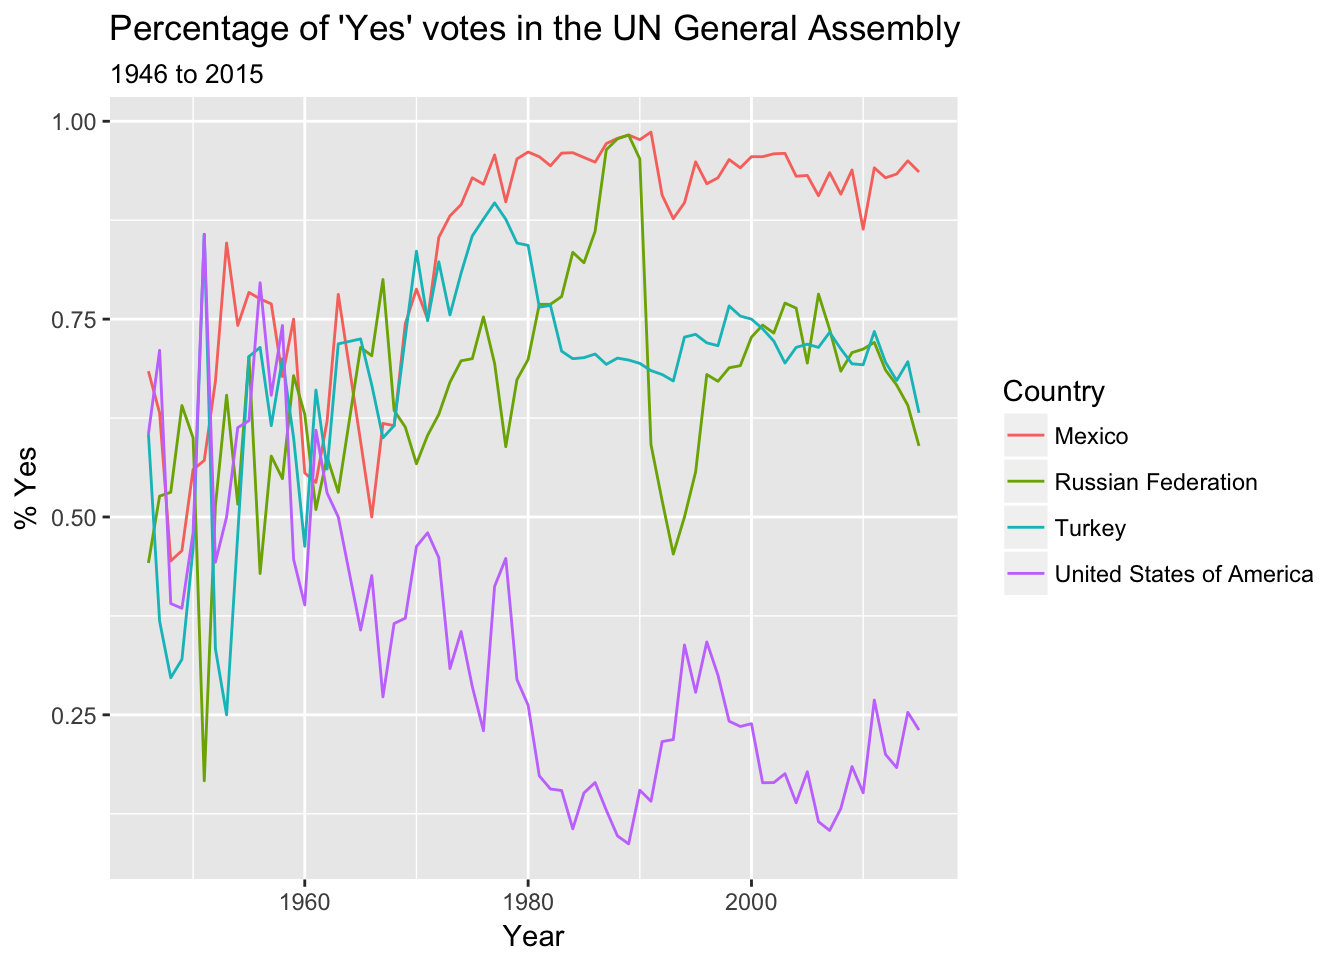
\includegraphics[width=0.7\linewidth]{02-dayone_files/figure-latex/plot-yearly-yes-1} \end{center}

And then, we create a visualization that compares how the voting record
of the United States changed over time on a variety of issues, and
compare it to another country.

\begin{Shaded}
\begin{Highlighting}[]
\NormalTok{un_votes }\OperatorTok
\StringTok{  }\KeywordTok{filter}\NormalTok{(country }\OperatorTok\StringTok{ }\KeywordTok{c}\NormalTok{(}\StringTok{"United States of America"}\NormalTok{, }\StringTok{"Turkey"}\NormalTok{)) }\OperatorTok
\StringTok{  }\KeywordTok{inner_join}\NormalTok{(un_roll_calls, }\DataTypeTok{by =} \StringTok{"rcid"}\NormalTok{) }\OperatorTok
\StringTok{  }\KeywordTok{inner_join}\NormalTok{(un_roll_call_issues, }\DataTypeTok{by =} \StringTok{"rcid"}\NormalTok{) }\OperatorTok
\StringTok{  }\KeywordTok{group_by}\NormalTok{(country, }\DataTypeTok{year =} \KeywordTok{year}\NormalTok{(date), issue) }\OperatorTok
\StringTok{  }\KeywordTok{summarize}\NormalTok{(}
    \DataTypeTok{votes =} \KeywordTok{n}\NormalTok{(),}
    \DataTypeTok{percent_yes =} \KeywordTok{mean}\NormalTok{(vote }\OperatorTok{==}\StringTok{ "yes"}\NormalTok{)}
\NormalTok{    ) }\OperatorTok
\StringTok{  }\KeywordTok{filter}\NormalTok{(votes }\OperatorTok{>}\StringTok{ }\DecValTok{5}\NormalTok{) }\OperatorTok\StringTok{  }\CommentTok{# only use records where there are more than 5 votes}
\StringTok{  }\KeywordTok{ggplot}\NormalTok{(}\DataTypeTok{mapping =} \KeywordTok{aes}\NormalTok{(}\DataTypeTok{x =}\NormalTok{ year, }\DataTypeTok{y =}\NormalTok{ percent_yes, }\DataTypeTok{color =}\NormalTok{ country)) }\OperatorTok{+}
\StringTok{    }\KeywordTok{geom_point}\NormalTok{() }\OperatorTok{+}
\StringTok{    }\KeywordTok{geom_smooth}\NormalTok{(}\DataTypeTok{method =} \StringTok{"loess"}\NormalTok{, }\DataTypeTok{se =} \OtherTok{FALSE}\NormalTok{) }\OperatorTok{+}
\StringTok{    }\KeywordTok{facet_wrap}\NormalTok{(}\OperatorTok{~}\StringTok{ }\NormalTok{issue) }\OperatorTok{+}
\StringTok{    }\KeywordTok{labs}\NormalTok{(}
      \DataTypeTok{title =} \StringTok{"Percentage of 'Yes' votes in the UN General Assembly"}\NormalTok{,}
      \DataTypeTok{subtitle =} \StringTok{"1946 to 2015"}\NormalTok{,}
      \DataTypeTok{y =} \StringTok{"% Yes"}\NormalTok{,}
      \DataTypeTok{x =} \StringTok{"Year"}\NormalTok{,}
      \DataTypeTok{color =} \StringTok{"Country"}
\NormalTok{    )}
\end{Highlighting}
\end{Shaded}

\begin{center}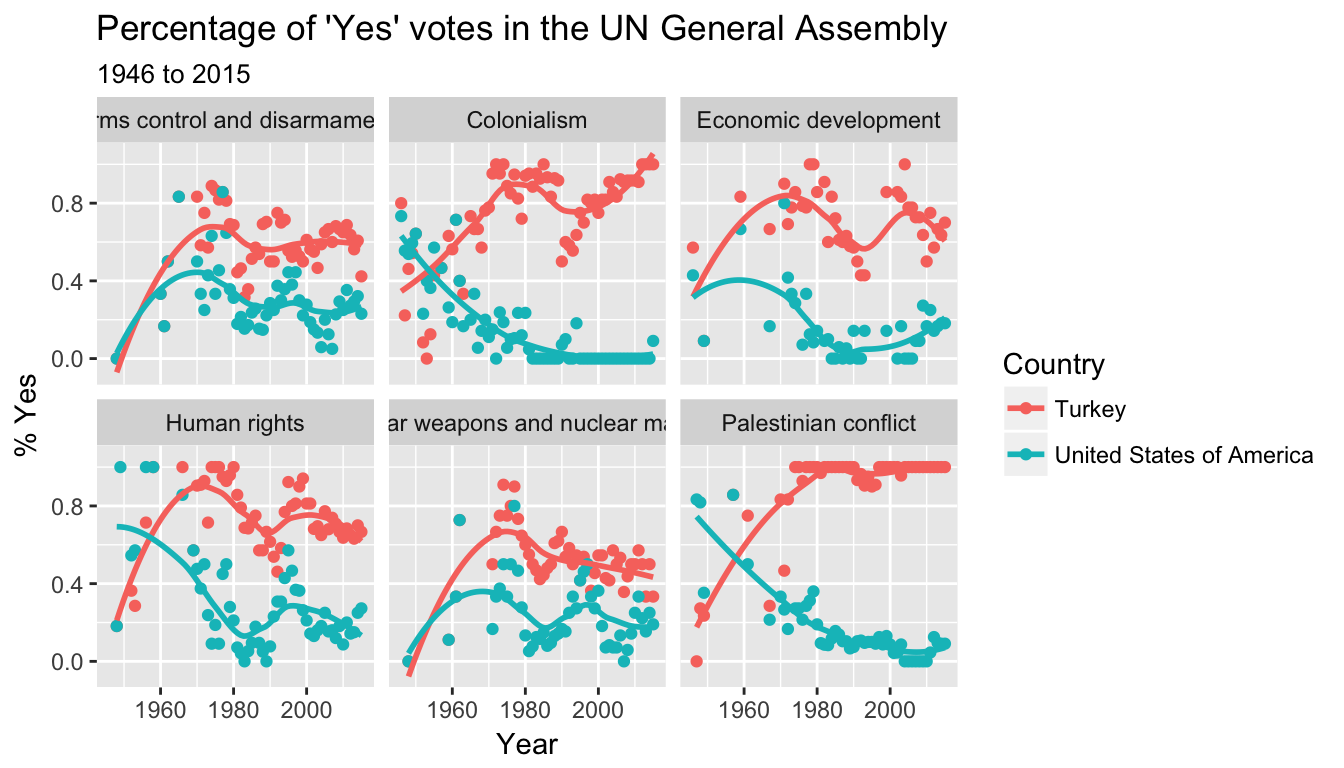
\includegraphics[width=0.7\linewidth]{02-dayone_files/figure-latex/plot-yearly-yes-issue-1} \end{center}

At this point, instead of a formal introduction on R syntax, I recommend
letting students change parameters passed to these functions, such as
which countries are being plotted, and reknit the document to view the
changes.

{[}TO DO: Find a good way to insert slides.{]}

Link to relevant slides:
\url{https://github.com/rstudio-education/datascience-box/tree/master/slides/p0_d01-welcome}

\chapter{Meet the toolkit}\label{toolkit}

\section{\ldots{}}\label{section}

\part{Exploring data}\label{part-exploring-data}

\chapter{Introduction}\label{explore-intro}

This is where into to part 1 goes.

\chapter{Data visualization}\label{data-viz}

Some words.

Then embed slides:
\href{https://github.com/rstudio-education/datascience-box/tree/master/slides/p1_d01-data-viz}{Visualizing
data}

Link to lab:
\href{https://github.com/rstudio-education/datascience-box/blob/master/labs/lab-02-data-wrangle-visualize.Rmd}{Data
wrangling and visualization}

And to HW:
\href{https://github.com/rstudio-education/datascience-box/blob/master/assignments/hw-02.Rmd}{Gotta
catch 'em all}

\part{Making rigorous
conclusions}\label{part-making-rigorous-conclusions}

\chapter{Introduction}\label{rigor-intro}

This is where into to part 2 goes.

\part{Looking forward}\label{part-looking-forward}

\chapter{Introduction}\label{forward-intro}

This part has a bunch of independent modules, each on a different topic.
Pick and choose to your liking, depending on how much time you have to
cover them.

\part{Infrastructure}\label{part-infrastructure}

\chapter{Introduction}\label{infra-intro}

Intro to part 4 goes here.

\bibliography{book.bib,packages.bib}


\end{document}
